\documentclass[12pt]{article}
\usepackage{pgfplotstable}
\usepackage[a4paper,margin=1in,landscape]{geometry}

\title{\bfseries Cup cooling experiment with Arduino}
\date{}
\begin{document}
\maketitle
\thispagestyle{empty}

\noindent
\textbf{Equipment}: \texttt{The K-type thermocouple with digital amplifier on the MAX6675 chip.}

\begin{center}
%---------------------------------------------------------
\begin{minipage}[]{0.45\linewidth}\centering
    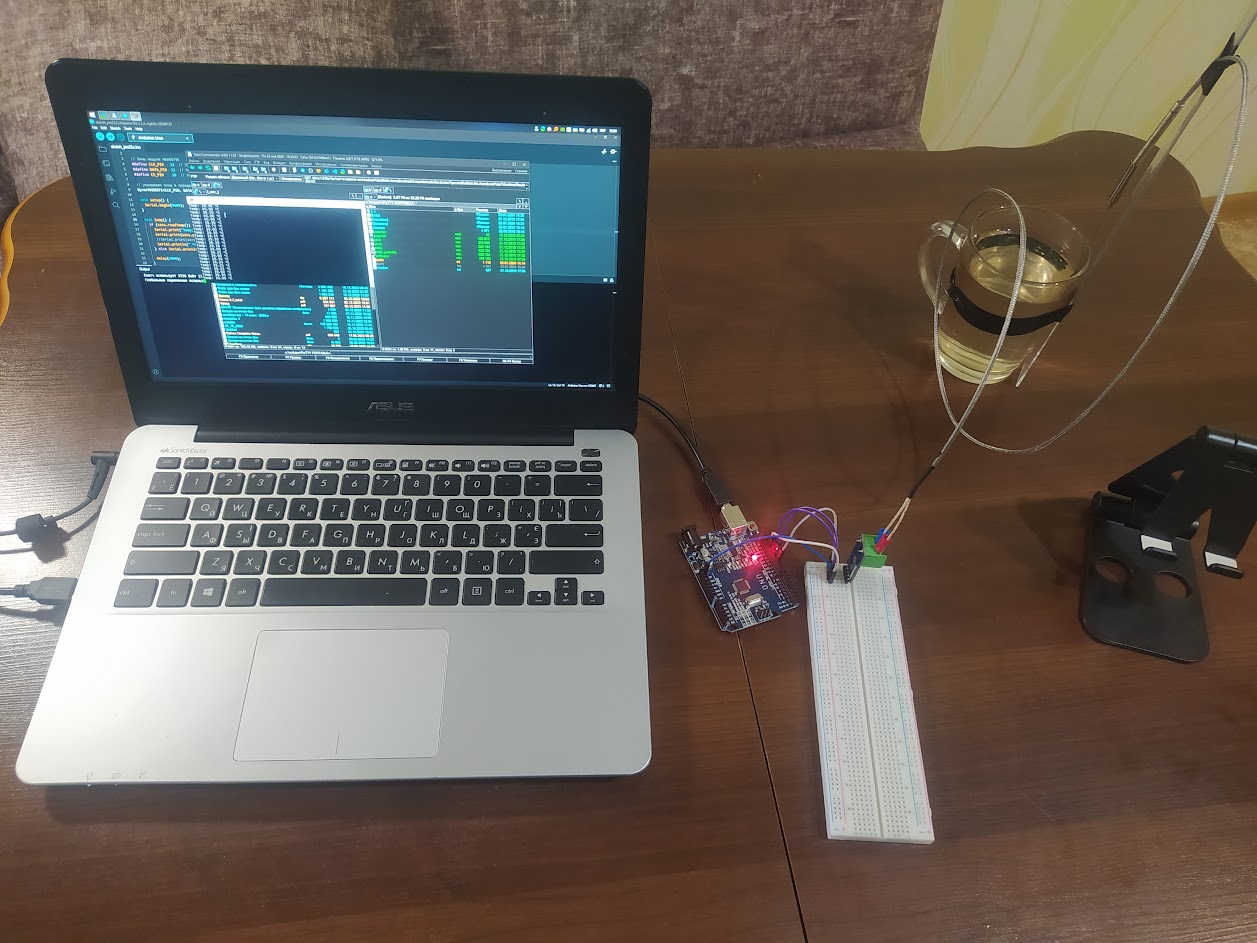
\includegraphics[width=\linewidth]{cooling.png}
\end{minipage}%
\quad
%---------------------------------------------------------
\begin{minipage}[]{0.45\linewidth}\centering
    \begin{tikzpicture}
    \begin{axis}[%
    title={Cooling a cup of tea},
    width=\linewidth,
    height=0.75\linewidth,
    			xlabel={$t$ / min},
    			ylabel={$T$ / ${^\circ}$C},
    scale only axis,
    enlargelimits=false,
    line join=round,
    % === Налаштування сітки ===
    grid = both,
    grid style={line width=.1pt, draw=gray!10},
    major grid style={line width=.2pt,draw=gray!50},
    minor tick num = 5,
    minor grid style = {line width=.1pt,draw=gray!10},
    ]
    \addplot [color=red, line width=1pt, mark=*, mark size=1pt] table [x expr=\coordindex * 5 / 60, y=y] {data.txt};

%    \addplot[domain=0:45, blue, ultra thick] {25 + (90  - 25)*exp(-0.045*x^0.94)};
    \node[anchor=south east,
    		draw=none,
    		fill=white,
            font=\ttfamily\small,
    		align=left,
    		fill opacity=0.5,
    		text opacity=1,
    		] at ([shift ={(0cm,7cm)}]current axis.south east) {
    		Room temperature: $T_0 = 23^\circ$C\\
            Systematic absolute error of the sensor: $\pm 0.25^\circ$C
            };

    \end{axis}

    \end{tikzpicture}
\end{minipage}
%---------------------------------------------------------
\end{center}

\end{document}
